\documentclass[a4paper]{article}

\usepackage{color}
\usepackage{url}
\usepackage[T2A]{fontenc} 
\usepackage[utf8]{inputenc}
\usepackage{graphicx}

\usepackage[english,serbian]{babel}
\usepackage[unicode]{hyperref}
\hypersetup{colorlinks,citecolor=red,filecolor=green,linkcolor=blue,urlcolor=blue}

\title{Slučajevi upotrebe Udruženja u okviru zaposlenih}


\begin{document}

\maketitle

\section{Slučajevi upotrebe}

\subsection{Udruženja}
\subsubsection{Slučaj upotrebe: Zahtev za osnivanje udruženja}
\begin{enumerate}
    \item \textbf{Kratak opis:} Zaposleni u kompaniji šalje zahtev za osnivanje udruženja.
    \item \textbf{Učesnici:}
        \begin{itemize}
            \item Zaposleni
        \end{itemize}
    \item \textbf{Preduslovi:} Sistem je u funkciji. Zaposleni ima pristup internetu i sistemu.
    \item \textbf{Postuslovi:} Zahtev za osnivanje udruženja je uspešno podnet i u statusu je čekanja za odobravanje. Vlasnik udruženja je obavešten.
    \item \textbf{Osnovni tok:}
        \begin{enumerate}
            \item Zaposleni otvara stranicu za udruženja.
            \item Klikom na dugme za osnivanje novog udruženja prikazuje se forma koja sadrži polje gde se bira tip udruženja.
            \item Za slučaj da je tip udruženja sportska sekcija, izvršava se podtok (a), za programersku sekciju podtok (b), a za ostalo podtok (c).
            \item Zaposleni popunjava formular.
            \item Zaposleni potvrđuje podnošenje zahteva.
            \item Sistem beleži zahtev za osnivanje udruženja i obaveštava Menadžere ljudskih resursa za validaciju.
        \end{enumerate}
    \item \textbf{Podtokovi:}
        \item Sportska sekcija
            \begin{enumerate}
                \item Zaposlenom se prikazuje forma gde se bira sport i polje gde se navode dodatne informacije.
            \end{enumerate}
        \item Programerska sekcija
            \begin{enumerate}
                \item Zaposlenom se prikazuje forma gde se unosi programski jezik za koji želi da osnuje zajednicu i polje gde se navode dodatne informacije.
            \end{enumerate}
        \item Ostalo
            \begin{enumerate}
                \item Zaposlenom se prikazuje forma gde se navodi naziv udruženja koji želi da osnuje, polje gde se navodi opis udruženja i polje gde se navode dodatne informacije.
            \end{enumerate}
    \item \textbf{Alternativni tokovi:}
        \begin{enumerate}
            \item \textbf{Formular nije ispravno popunjen.} Sistem obaveštava zaposlenog o greškama na formularu i vraća ga na korak (e).
        \end{enumerate}
    \item \textbf{Podtokovi:} /
    \item \textbf{Specijalni zahtevi:} /
    \item \textbf{Dodatne informacije:} /
\end{enumerate}

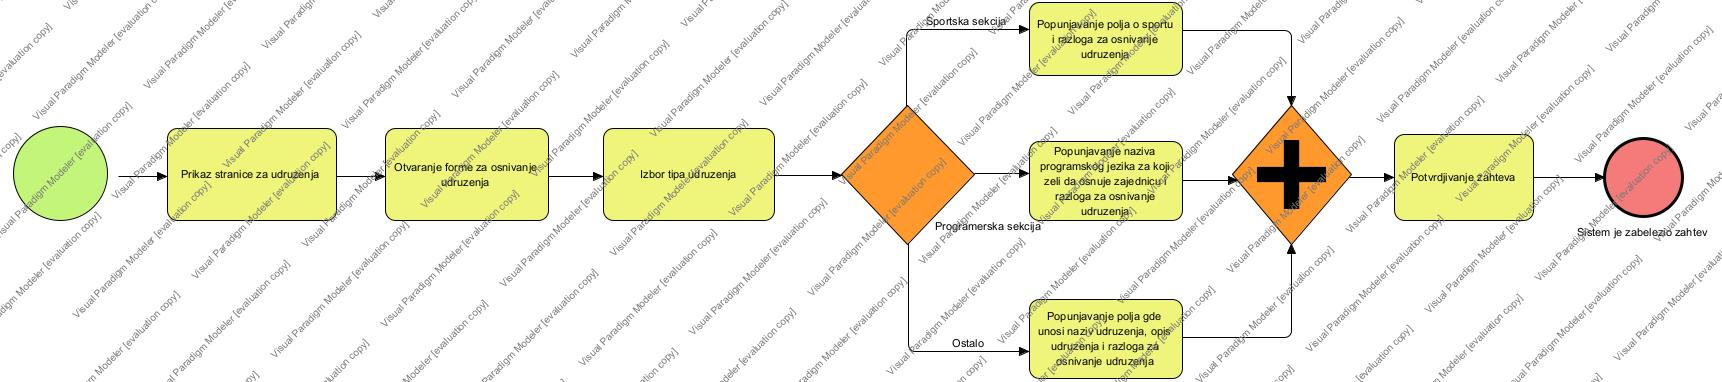
\includegraphics[width=\textwidth,height=\textheight,keepaspectratio]{BPMN/ZahtevZaOsnivanjeUdruzenja.jpg}

\subsubsection{Slučaj upotrebe: Zahtev za članstvo u udruženju}
\begin{enumerate}
    \item \textbf{Kratak opis:} Zaposleni u kompaniji šalje zahtev za članstvo u određenom udruženju unutar kompanije.
    \item \textbf{Učesnici:}
        \begin{itemize}
            \item Zaposleni
        \end{itemize}
    \item \textbf{Preduslovi:} Sistem je u funkciji. Zaposleni ima pristup internetu i sistemu.
    \item \textbf{Postuslovi:} Zahtev za članstvo je uspešno podnet. Vlasnik udruženja je obavešten.
    \item \textbf{Osnovni tok:}
        \begin{enumerate}
            \item Zaposleni otvara stranicu za udruženja.
            \item Sistem prikazuje listu svih postojećih udruženja.
            \item Zaposleni otvara stranicu udruženja za koje želi podneti zahtev za članstvo.
            \item Zaposleni otvara stranicu za članstvo u udruženju.
            \item Zaposleni se prijavljuje za članstvo pritiskom na dugme Želim da Postanem Član.
            \item Zaposleni potvrđuje podnošenje zahteva.
            \item Sistem beleži zahtev za članstvo i obaveštava vlasnika udruženja.
        \end{enumerate}
    \item \textbf{Alternativni tokovi:} /
    \item \textbf{Podtokovi:} /
    \item \textbf{Specijalni zahtevi:} /
    \item \textbf{Dodatne informacije:} /
\end{enumerate}

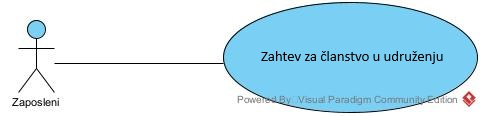
\includegraphics[scale=0.5]{UML/SlucajUpotrebe_Clanstvo.jpg}

\subsubsection{Slučaj upotrebe: Zahtev za održavanje događaja}
\begin{enumerate}
    \item \textbf{Kratak opis:} Zaposleni koji ima ulogu vlasnika udruženja šalje zahtev za održavanje događaja.
    \item \textbf{Učesnici:}
        \begin{itemize}
            \item Zaposleni
        \end{itemize}
    \item \textbf{Preduslovi:} Sistem je u funkciji. Zaposleni ima pristup internetu i sistemu.
    \item \textbf{Postuslovi:} Zahtev za održavanje događaja je podnet.
    \item \textbf{Osnovni tok:}
        \begin{enumerate}
            \item Zaposleni otvara stranicu za udruženja.
            \item Sistem prikazuje listu svih postojećih udruženja.
            \item Zaposleni otvara stranicu udruženja čiji je on vlasnik.
            \item Zaposleni otvara stranicu za podnošenje zahteva za održavanje događaja.
            \item Zaposleni popunjava formular za zahtev.
            \item Zaposleni potvrđuje podnošenje zahteva.
            \item Sistem beleži zahtev za održavanje događaja.
        \end{enumerate}
    \item \textbf{Alternativni tokovi:}
        \begin{enumerate}
            \item \textbf{Formular nije ispravno popunjen.} Sistem obaveštava zaposlenog o greškama na formularu i vraća ga na korak (e).
        \end{enumerate}
    \item \textbf{Podtokovi:} /
    \item \textbf{Specijalni zahtevi:} /
    \item \textbf{Dodatne informacije:} Formular za održavanje dogadjaja sadrži obavezna polja: naziv, opis, termin održavanja.
\end{enumerate}

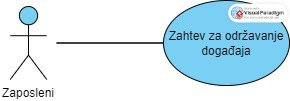
\includegraphics[scale=0.5]{UML/SlucajUpotrebe_OdrzavanjeDogadjaja.jpeg}

\subsubsection{Slučaj upotrebe: Zahtev za prisustvo događaju}
\begin{enumerate}
    \item \textbf{Kratak opis:} Zaposleni u kompaniji šalje zahtev za prisustvo događaju organizovanom od strane već postojeće zajednice u kompaniji.
    \item \textbf{Učesnici:}
        \begin{itemize}
            \item Zaposleni
        \end{itemize}
    \item \textbf{Preduslovi:} Sistem je u funkciji. Zaposleni ima pristup internetu, sistemu.
    \item \textbf{Postuslovi:} Zaposleni se uspešno prijavio za prisustvo događaju. Vlasnik zajednice je obavešten.
    \item \textbf{Osnovni tok:}
        \begin{enumerate}
            \item Zaposleni otvara stranicu za udruženja.
            \item Sistem prikazuje listu svih postojećih udruženja
            \item Zaposleni otvara stranicu udruženja za čiji događaj je zainteresovan
            \item Zaposleni otvara stranicu svih događaja udruženja
            \item Zaposleni bira događaj kome želi da prisustvuje
            \item Zaposleni se prijavljuje za događaj pritiskom na dugme Želim da Prisustvujem
            \item Sistem prikazuje da je prijava uspešna 
        \end{enumerate}
    \item \textbf{Alternativni tokovi:}
        \begin{enumerate}
            \item \textbf{Prijave za događaj su zatvorene.} Sistem obaveštava korisnika da je prijavljivanje zatvoreno. Sistem vraća korisnika na korak (d)
        \end{enumerate}
    \item \textbf{Podtokovi:} /
    \item \textbf{Specijalni zahtevi:} /
    \item \textbf{Dodatne informacije:} /
\end{enumerate}

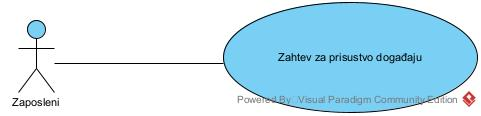
\includegraphics[scale=0.5]{UML/SlucajUpotrebe_PrisustvoDogadjaju.jpg}

\end{document}